\documentclass{beamer}

\usepackage[ngerman]{babel}
\usepackage[utf8x]{inputenc}
\usepackage{amsmath,amsfonts,amssymb}
\usepackage{tikz}
\usepackage{graphicx}

\usetikzlibrary{shapes,arrows,positioning,hobby,decorations.markings,fit,backgrounds,calc}

%\usetheme{Singapore}
\setbeamercovered{transparent}

\setbeamertemplate{section in toc}[sections numbered]
\setbeamertemplate{subsection in toc}[subsections numbered]
\setbeamertemplate{subsubsection in toc}[subsubsections numbered]

\newcommand\subsectnum{%
  \number\numexpr \insertpagenumber-\insertsubsectionstartpage+1\relax.~%
}

\begin{document}
\title{Projekt Straßenschilderkennung}   
\author{Artem Prokop\\
Theodor Malaki\\
Eike Florian Petersen} 
\date{\today} 

\frame{\titlepage} 
%
%\frame{\frametitle{Inhaltsverzeichnis}\tableofcontents} 
%
%
%\section {Vorstellung des Teams}
%\frame {\frametitle{\thesection. \insertsection}
%\begin{tabular}{l l}
%\hline
%\textbf{Name} & \textbf{Rolle/Aufgabenbereich} \\
%\hline
%Artem Prokop & Vorführung\\ 
%~ & Schilderkennung\\
%~\\
%Eike Florian Petersen & Vortrag \\
%~ & Farbsegmentierung, Floadfill\\
%~\\
%Theodor Malaki & Dokumentation \\
%~ & Formerkennung\\
%\end{tabular}
%}


\section {Projektdefinition}
\frame {\frametitle{\thesection. \insertsection}
Der Aufbau der Bilderkennung soll anhand des Papers ``A Robust Algorith for Detection and Classification of Traffic Signs in Video Data'' von Tanh Bui-Minh, Ovidiu Ghita, Paul F.Whelan and Trang Hoang umgesetzt werden.
\newline
\newline
\newline
\begin{tabular}{l l}
Eingabeformat: & Einzelbild \\
Ausgabeformat: & Bildliche Darstellung der Fundstelle/n \\
 & und textuelle Beschreibung der gefundenen Objekte \\
\end{tabular}
}

\section {Umsetzung}
\frame {\frametitle{\thesection. \insertsection}
% define block styles
\tikzstyle{block} = [rectangle,fill=gray!10,draw,text width=10em,text centered,minimum height=3em]
\tikzstyle{cloud} = [ellipse, fill=gray!10,draw, text width=5em, text centered, minimum height=3em]
\tikzstyle{line} = [draw, -latex']
\centering
\resizebox{0.66\linewidth}{!}{%
  \begin{minipage}{\linewidth}
      \begin{tikzpicture}[->,>=stealth', auto, node distance=1cm, main node/.style={circle,fill=blue!15,draw,font=\sffamily\bfseries}]
      % place nodes
      \node [block, text width=13em] (1) {\centering Einzelbild lesen};
      \node [block, below of = 1, node distance=1.5cm, text width=13em] (2) {Farbsegmentierung};
      \node [block, below of = 2, node distance=1.5cm, text width=13em] (3) {Flood fill / Flächen finden};
      \node [block, below of = 3, node distance=1.5cm, text width=13em] (4) {Formerkennung};
      \node [block, below of = 4, node distance=1.5cm, text width=13em] (5) {Klassifizierung};
      \node [block, below of = 5, node distance=1.7cm, text width=13em] (7) {Einzelbild schreiben \\ textuelle Dokumentation erzeugen};
      
      \path [line] (1) -- (2);
      \path [line] (2) -- (3);
      \path [line] (3) -- (4);
      \path [line] (4) -- (5);
      \path [line] (5.east) [bend right=50] to node[pos=.5,xshift=4cm]{für ROT, BLAU, GELB} (2.east);
      \path [line] (5) -- (7);
      
      \end{tikzpicture}
  \end{minipage}
  }
}


\frame {\frametitle{\thesection. \insertsection}
\textbf{Farbsegmentierung}
{
\centering 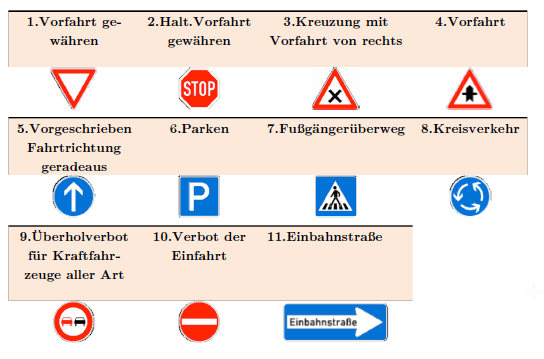
\includegraphics[width=10cm]{Schilder}\\~\\
}
}


\subsection {Bild vorbereiten}
\frame {\frametitle{\thesection.\thesubsection~ \insertsubsection}
% define block styles
\begin{itemize}
\item Farbsegmentierung für (aktuelle Farbe ROT, BLAU)\\
\begin{itemize}
\item Für jeden Pixel wird das Verhältnis der Farbe zur Addition der drei Farben bestimmt\\
\item Ist das Verhältnis pos. Pixel weiß, ansonsten schwarz
\end{itemize}
\item Flood fill zur Bereichsfindung\\
\begin{itemize}
\item Bereiche \textless 100 Pixel werden eleminiert, da eine Schilderkennung hier nicht möglich ist.\\~\\
Aus dem Paper: height \textgreater 30 Pixeln vorgegeben mit einer Breite von min. ~ 3 - 4 Pixeln
\end{itemize}
\end{itemize}
}

\frame {\frametitle{\thesection.\thesubsection~ \insertsubsection}
\textbf{Farbsegmentierung}
{
\centering 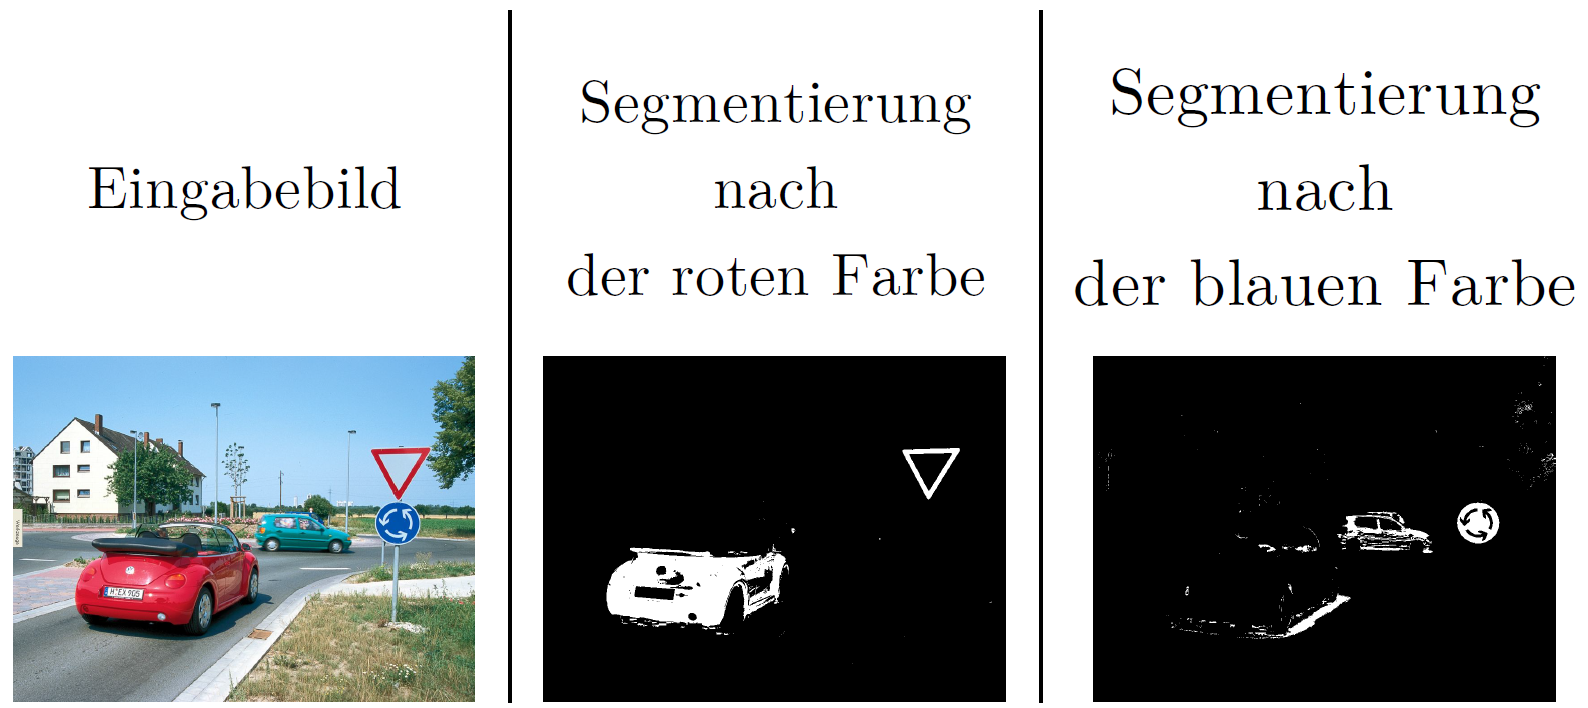
\includegraphics[width=10cm]{Autos}\\~\\
}
}

\subsection {Formerkennung}
\frame {\frametitle{\thesection.\thesubsection~ \insertsubsection}
\begin{tabular}{l l l}
\hline
\textbf{Farbe} & \textbf{Form} & \textbf{Kategorie} \\
\hline
Rot & Oktagonal & Stop \\ 
Rot & Dreieck, Spitze unten & Vorfahrt gewähren \\ 
Rot & Dreieck, Spitze oben & Warnung \\ 
Rot & Kreis & Verbot \\ 
Blau & Kreis & Verpflichtend \\
Blau & Viereck & Hinweis \\
\end{tabular}
\textbf{Bildausschnitt bereinigen}\\
\centering 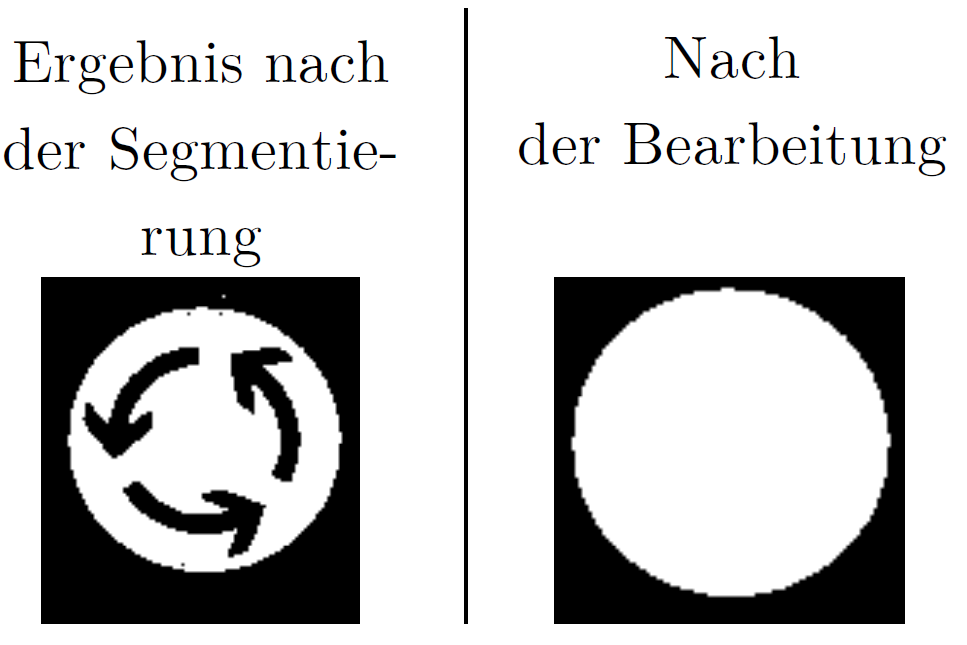
\includegraphics[width=6cm]{Bereinigen}\\~\\
}

\frame {\frametitle{\thesection.\thesubsection~ \insertsubsection}
\textbf{Berechnung nach Paper}\\
Invariante\\
{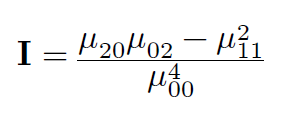
\includegraphics[width=2cm]{Invariante}\\}
Momente\\
{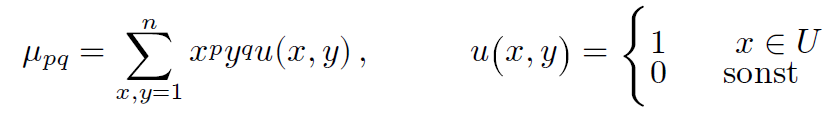
\includegraphics[width=7cm]{Momente}\\}
Auswertung\\
{\centering 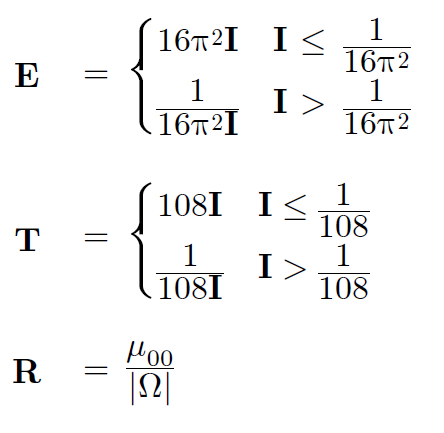
\includegraphics[width=3cm]{Auswertung}} \tiny
\begin{itemize}
\item $Rund : 0.98~\textless ~E \le 1$
\item $Achteck : 0.98~\textless ~E \le 1~ UND~0.7~\textless ~R \le 1$
\item $Dreieckig : 0.97~\textless ~T \le 1$
\item $Viereckig : 0.7~\textless ~R \le 1$
\end{itemize}
}

\frame {\frametitle{\thesection.\thesubsection~ \insertsubsection}
\textbf{Berechnung nach Paper}\\
{\centering 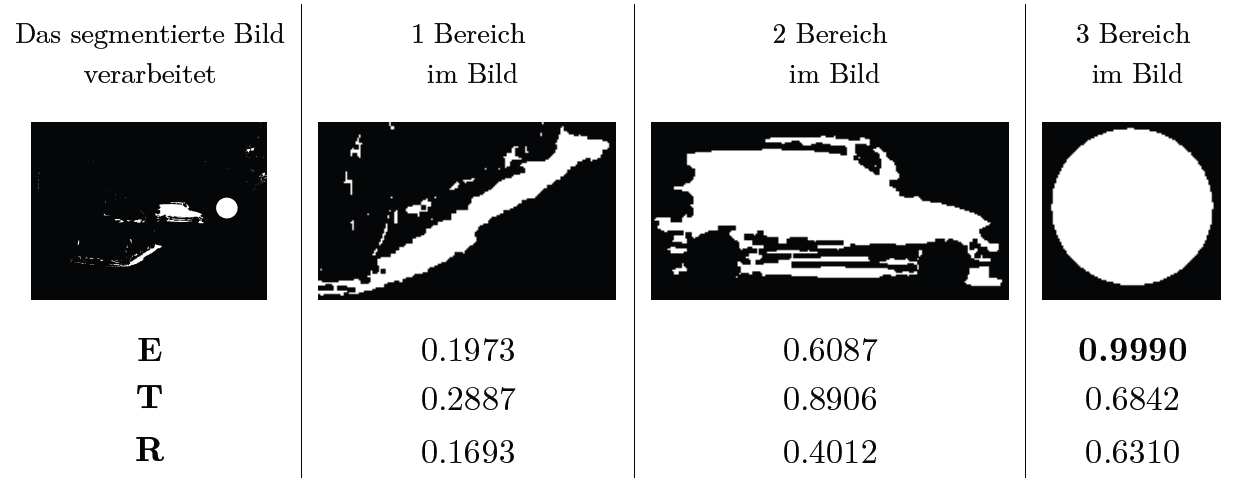
\includegraphics[width=10cm]{Bereiche}\\~\\}
}

\subsection {Klassifizierung}
\frame {\frametitle{\thesection.\thesubsection~ \insertsubsection}
Nach der Formerkennung bleiben nur noch wenige Verkehrszeichen die untereinander verglichen werden müssen.\\
\begin{itemize}
\item Skalierung und Endzerrung des Bildes auf 80 x 80
\item Linienprofil erstellen (Position in Katalog definiert)
\item Hoch / Tiefpunktwechsel vergleichen
\end{itemize}
~\\
{\centering 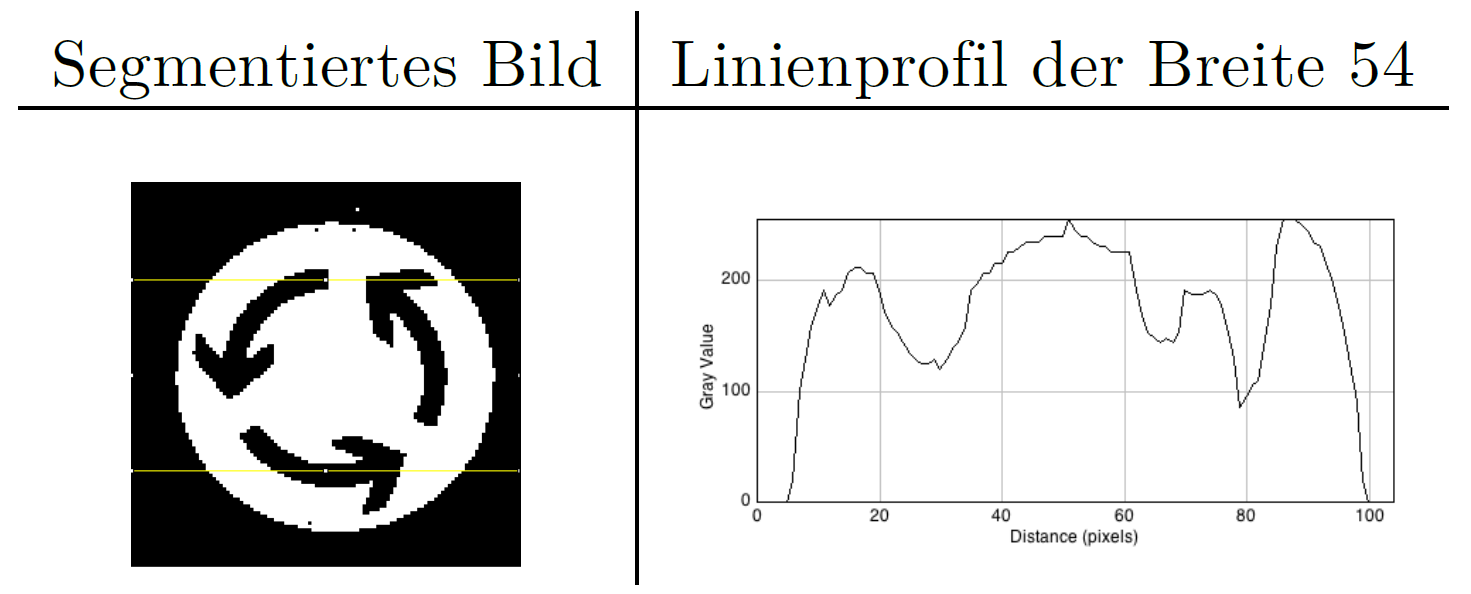
\includegraphics[width=10cm]{Linienprofil}\\}
}

\subsection {Ergebnis}
\frame {\frametitle{\thesection.\thesubsection~ \insertsubsection}
{\centering 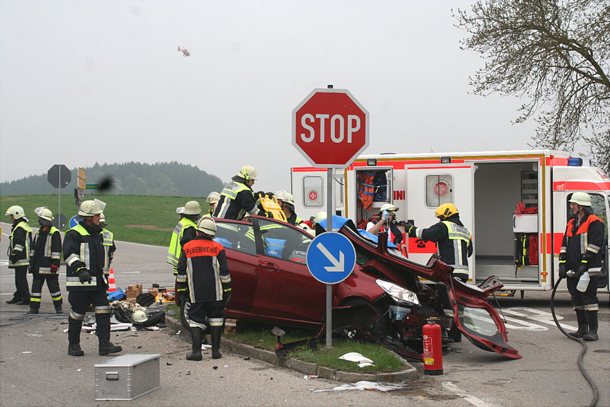
\includegraphics[width=6cm]{014-IMG_6852_610}\\}
{\centering 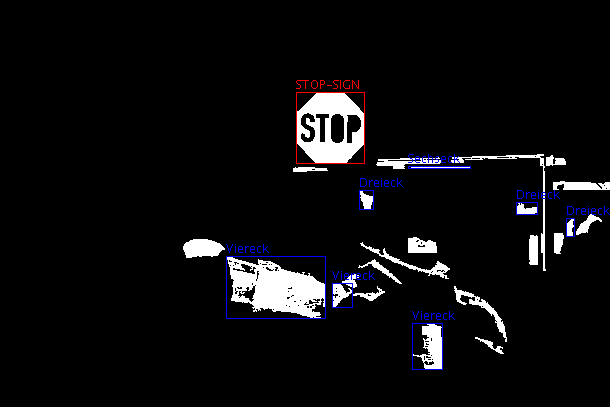
\includegraphics[width=6cm]{segmentedRed}\\}
}

\subsection {Verbesserungen}
\frame {\frametitle{\thesection.\thesubsection~ \insertsubsection}
\begin{itemize}
\item Bild mit geringerer Auflösung zur Erkennung erstellen
\item Endgültige Schilderkennung anhand von Skeletten/Neuronale Netze
\item Drehung von Schildern / Falschschilderkennung an Kreuzungen (Fahrbahnerkennung)
\item Two Path Filter anstelle von Flood fill (Vortrag von gerade eben)
\end{itemize}
}

\end{document}

